
\section{An Illustrative Example}
\label{illustrative-example}


%% Loading and unloading costs no fuel, while driving costs between 1 and
%% 5 fuels units (as indicated by edge labels).\\ The amount of fuel
%% available is 1.5 times higher than needed to deliver all packages;
%% concretely, the initial fuel in trucks is $fuel(T_0) = 16$, $fuel(T_1)
%% = 7$.

To illustrate our approach and the kind of explanations it provides,
consider the IPC NoMystery domain, a classical transportation domain
with fuel consumption. We consider the example task with two trucks
and three packages as illustrated below. Fuel costs are indicated at
road segments (initial fuel is $16$ for $T_0$ and $7$ for $T_1$). The
packages are initially at $L_0$ (shown in blue); their goal locations
are $L_4$, $L_3$,and $L_5$ (shown in red). We define three kinds %
%
\begin{wrapfigure}{r}{0.4\columnwidth}
\vspace{-0.3cm} \hspace{-0.7cm} 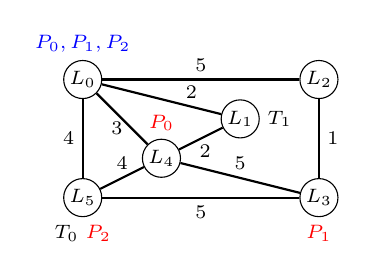
\begin{tikzpicture}[scale=0.5]
	\scriptsize
  \node[draw, circle, inner sep=1pt, label=above:{\textcolor{blue}{$P_0, P_1,P_2$}}] (l0) at (0,0) {$L_0$};
  \node[draw, circle, inner sep=1pt, label=right:{$T_1$}] (l1) at (4,-1) {$L_1$};
  \node[draw, circle, inner sep=1pt] (l2) at (6,0) {$L_2$};
  \node[draw, circle, inner sep=1pt, label=below:{\textcolor{red}{$P_1$}}] (l3) at (6,-3) {$L_3$};
  \node[draw, circle, inner sep=1pt, label=above:{\textcolor{red}{$P_0$}}] (l4) at (2,-2) {$L_4$};
  \node[draw, circle, inner sep=1pt, label=below:{$T_0$ \textcolor{red}{$P_2$}}] (l5) at (0,-3) {$L_5$};

  \draw[thick] (l0) to node[above] {5} (l2);
  \draw[thick] (l0) to node[above, pos=0.75] {2} (l1);
  \draw[thick] (l0) to node[below, pos=0.4] {3} (l4);
  \draw[thick] (l0) to node[left] {4} (l5);
  \draw[thick] (l2) to node[right] {1} (l3);
  \draw[thick] (l4) to node[below, pos=0.6] {2} (l1);
  \draw[thick] (l4) to node[above] {5} (l3);
  \draw[thick] (l5) to node[below] {5} (l3);
  \draw[thick] (l4) to node[above] {4} (l5);
\end{tikzpicture}
%% \vspace{-0.25cm} \hspace{-0.6cm} \caption{Illustrative IPC NoMystery example.}
%% \label{fig:nomystery-example}
\vspace{-0.3cm}
\end{wrapfigure}
%
of action-set properties for this domain:
\emph{uses $T_i$ $(L_x,L_y)$} (truck $T_i$ drives at least once from
$L_x$ to $L_y$ or vice versa); \emph{doesn't use $T_i$ $(L_x,L_y)$}
(the opposite); \emph{same truck $P_x$ $P_y$} (both packages are
delivered by the same truck). In our example task, we consider six
instances of these properties: 1.\ uses $T_0$ $(L_2,L_3)$; 2.\ same
truck $P_1$ $P_2$; 3.\ uses $T_0$ $(L_4,L_3)$; 4.\ same truck $P_2$
$P_0$; 5.\ doesn't use $T_0$ $(L_0,L_5)$; 6.\ uses $T_1$ $(L_5,L_4)$.

We fix the package destinations as hard goals, defining the set of
plans \plans\ considered. Computing the MUGS over the six action-set
properties using the algorithms previously described, it turns out
there are seven minimal unsolvable subsets of these properties, each
of size three.

Say now that the current plan uses $T_0$ only, and includes the action
(drive T0 L5 L0). The user might ask \emph{''Why don't you avoid the
  road $L_0-L_5$, which has a lot of traffic at the
  moment?''}. Answering this question in terms of contrastive
explanation, as previously discussed, corresponds to forcing property
5 to be satisfied. At the same time, the plan already satisfies
properties 2 and 4. However, one of the MUGS is $\{2,4,5\}$, and hence
the answer to the user question would be: \textit{Because if you don't
  use that road, then you would not be able to deliver all packages
  using a single truck}.
